\chapter{Verwandte Arbeiten} \label{sec:VerwandteArbeiten}
Im Folgenden werden Forschungsarbeiten vorgestellt, die sich mit Fragestellung beschäftigen, die den beiden zuvor vorgestellten Problemstellungen (siehe Abschnitt \ref{sec:Problemstellung}) ähnlich sind. Zunächst wird ein Überblick über Arbeiten gegeben, die sich mit dem Vergleich oder Vorstellung mehrerer Visualisierungstechniken beschäftigen. Anschließend werden Arbeiten vorgestellt, die sich speziell mit dem Treemap-Problem beschäftigen, also dem Problem von verschwindenden Knoten.




\subsection{Vergleich von Visualisierungstechniken} \label{sec:VergleichVisualisierungstechniken}

Die Arbeit von Pacione et al. (\textit{A comparative evaluation of dynamic visualisation tools} \cite{pacione2003comparative}) vergleicht fünf dynamische Visualisierungstools bezüglich ihrer Eignung für das Softwareverständnis und das Reverse Engineering. Die Autoren verfolgen das Ziel, Gründe dafür zu identifizieren, weshalb der Einsatz dieser Werkzeuge außerhalb der Forschung bislang nur begrenzt erfolgt, obwohl sie großes Potenzial für die Analyse komplexer Softwaresysteme bieten. Die Studie macht deutlich, dass keines der untersuchten Tools alle Anforderungen an Softwareverständnis vollständig abdeckt. Insbesondere wird auf Defizite in der Abbildung von Design-Patterns und Hotspot-Analysen hingewiesen, was unter Anderem im Kontext der Evaluation in dieser Arbeit untersucht werden soll.

Einen Überblick im Bereich der dreidimensionalen Softwarevisualisierung gibt die Arbeit von Teyseyre et al. (\textit{An overview of 3D software visualization} \cite{overview3D}). Die Autoren präsentieren verschiedene Visualisierungsansätze und Werkzeuge. Dabei werden folgende Kategorien differenziert:
\begin{itemize}
\item \textbf{Graphbasierte Ansätze:} 3D-Knoten-Kanten-Diagramme mit Fokus auf die Darstellung von Klassenbeziehungen
\item \textbf{Baumstrukturen:} Dreidimensionale Variationen wie \textit{Cone Trees}, \textit{Information Cubes} (im Grund 3D Treemaps) oder \textit{hierarchical nets} (siehe Abbildung \ref{fig:hierarchicalNet3D}) zur hierarchischen Darstellung von Softwareelementen
\item \textbf{Abstrakte Geometrische Darstellungen:} Nutzung von verschiedenen Formen zur Darstellung von verschiedenen Metriken und Strukturen. (Beispiel in Abbildung \ref{fig:geometrischeFiguren})
\end{itemize}
Sie zeigen auch auf, dass einige Ansätze Metaphern wie Städte oder Landschaften aus der echten Welt nutzen.
Interessant ist, dass von den 22 analysierten Tools nur vier für das Management oder Stakeholder ohne spezielle Entwicklungskompetenzen geeignet sind. Von diesen vier visualisiert zudem lediglich eines dieser Werkzeuge tatsächlich den Quellcode. Die anderen drei Tools konzentrieren sich auf die Visualisierung von Anforderungen. Zudem wird ein Mangel an empirischen Nutzungsstudien im 3D-Bereich konstatiert, was den Status und die Praxistauglichkeit der Ansätze weiter einschränkt. \cite{overview3D} In dieser Arbeit wird daher untersucht, ob die in dieser Arbeit vorgestellten Ansätze auch für Nutzer ohne tiefere technische Kenntnisse geeignet sind.

\begin{figure}
    \centering
    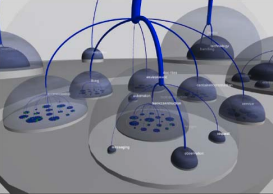
\includegraphics[width=0.8\textwidth]{images/verwandte/hierarchicalNet3D.png}
    \caption{Beispiel für ein hierarchisches Netz in 3D. Die hierarchische Struktur wird durch Kreise, Halbkugeln und deren Verbindungen dargestellt. \cite[6]{overview3D}}
    \label{fig:hierarchicalNet3D}
\end{figure}

\begin{figure}
    \centering
    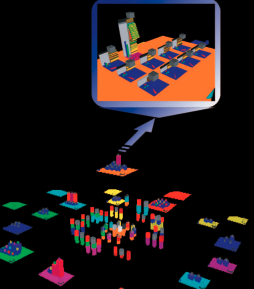
\includegraphics[width=0.8\textwidth]{images/verwandte/geometrischeFiguren.png}
    \caption{Beispiel für eine abstrakte geometrische Darstellung von Software. \cite[7]{overview3D}}
    \label{fig:geometrischeFiguren}
\end{figure}

Auch die Arbeit von Caserta und Zendra (\textit{Visualization of the static aspects of software: A survey} \cite{staticSurvey}) gibt einen Überblick über etablierte und aktuelle Visualisierungstechniken und ordnet diese unterschiedlichen Analyseebenen zu:
\begin{itemize}
\item \textbf{Quellcode-Ebene:} Zeilenorientierte Visualisierungen von einzelnen Dateien oder Klassen
\item \textbf{Klassen-/Mittel-Ebene:} Darstellungen der Strukturen oder Relationen von Dateien oder Klassen
\item \textbf{Architekturebene:} Globale Übersichten über Organisation und Qualitätsattribute, etwa durch Darstellung von Vererbungen und Aufrufstrukturen
\end{itemize}
Für die Architekturebene, die im Fokus dieser Arbeit steht, werden insbesondere folgende Visualisierungstypen diskutiert: Tree/Node-Link-Diagramme (wie Bereits in der Grundlagen gezeigt: bei großen Systemen schnell unübersichtlich), Treemaps und deren Varianten (Circular, Sunburst, Voronoi), die hierarchische Strukturen platzsparend repräsentieren und in 2D sowie 3D verfügbar sind. Sie stellen unter anderem folgende Probleme dieser Visualisierungen fest: Schlechte Nutzbarkeit, kognitive Überlastung, Desorientierung in dreidimensionalen Darstellungen sowie eine geringe Verbreitung praxistauglicher Tools, da viele existierende Lösungen im Prototypstatus sind.

Die Übersicht von Khan et al. (\textit{Visualization and evolution of software architectures} \cite{visualizationEvolution}) stellt ebenfalls verschiedene Visualisierungstechniken vor.
Sie unterscheiden zwischen hierarchischen und beziehungsorientierten Visualisationstechniken. Bei den hierarchischen Ansetzen werden platzfüllende Treemaps vorgestellt, die aufgrund ihrer Eigenschaften vor allem für große Hierarchien geeignet sind, wobei Sie hervorheben, dass Einschränkungen hinsichtlich der Visualisierung multipler Metriken und der Anschaulichkeit interner Strukturen bestehen, was in dieser Arbeit angegangen wird. Ergänzend nennen die Autoren auch Icicle Plots, Sunburst-Diagramme und hyperbolische Bäume (siehe Abbildung \ref{fig:dreiVis}).

\begin{figure}
    \centering
    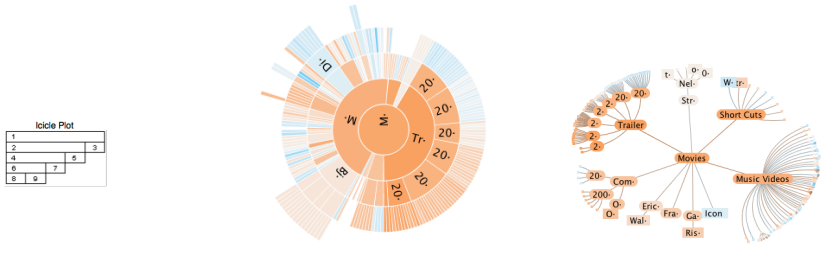
\includegraphics[width=0.8\textwidth]{images/verwandte/dreiVis.png}
    \caption{Beispiele für \textit{Icicle Plots} (links), \textit{Sunburst-Diagramme} (mitte) und \textit{hyperbolische Treelayouts} (rechts). \cite[4]{visualizationEvolution}}
    \label{fig:dreiVis}
\end{figure}

In \textit{Software visualization tools: survey and analysis} \cite{bassil2001software} von Bassil und Keller führen eine Umfrage durch, in der sie untersuchen, was Nutzern bei Softwarevisualisierungstools wichtig ist. Es zeigte sich, dass insbesondere hierarchische Repräsentationen, Benutzerfreundlichkeit und Skalierbarkeit bei großen Softwaresystemen von den Nutzern als entscheidend bewertet werden. Auch hier ist auffällig, dass speziell Experten befragt werden und sich auch die meisten untersuchten Werkzeuge primär an Experten und weniger an Endanwender wie Softwarekunden oder Management richten.

Eine detaillierte Übersicht verschiedener Treemap-Layout-Algorithmen geben Scheibel et al. in ihrer Arbeit \textit{Survey of treemap layout algorithms} \cite{scheibel2020survey}. Die Autoren unterscheiden Treemap-Algorithmen anhand der Art der Aufteilung (packing vs. splitting). Splitting ist die klassische Treemap-Variante, bei der die Fläche geteilt wird. Packing-Ansätze hingegen platzieren die Rechtecke so, dass sie möglichst wenig Platz verschwenden. Beide Ansätze erzeugen leicht Verschiedene Layouts (siehe Abbildung \ref{fig:packingVsSplitting}).  

\begin{figure}
    \centering
    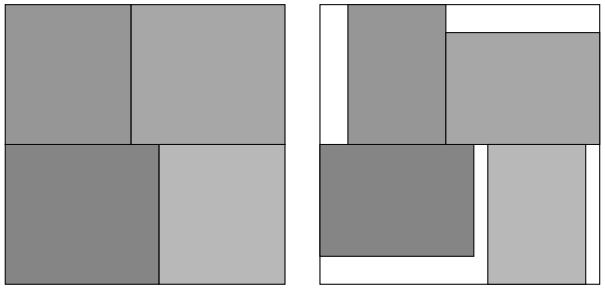
\includegraphics[width=0.8\textwidth]{images/verwandte/packingVsSplitting.png}
    \caption{Beispiel für Layouts die durch Splitting (links) und Packing (rechts) Algorithmen erzeugt wurden. Es ist zu erkennen, dass bei Packing-Algorithmen mehr Platz zwischen den Knoten entsteht. \cite[3]{scheibel2020survey}}
    \label{fig:packingVsSplitting}
\end{figure}

Zudem unterscheiden sie verschiedene layouts anhand der Layout-Form (z.,B. rechteckig, kreisförmig, konvex, nicht-konvex) sowie der Referenzraum-Dimension (2D vs. 3D). Für die in dieser Arbeit betrachteten Anwendungsfälle stehen rechteckige 2D-Splitting-Layouts im Vordergrund (siehe Abschnitt\ref{sec:Problemstellung} und \ref{sec:Treemap}) Wir stellen fest, dass von 81 analysierten Ansätzen sind 54 rechteckige und 58 splitting-basiert sind, was zeigt, dass dies das präferierte Treemap verfahren ist. 
Neben klassischen Verfahren (Slice-and-Dice, Squarified, Strip) werden auch Polygon-, Voronoi- und Circular-Treemaps sowie spezialisierte Layouts beschrieben, etwa für Aspektverhältnis-Optimierung oder Ordnungserhaltung. Die große Vielfalt verdeutlicht die Notwendigkeit einer gezielten anwendungsspezifischen Auswahl des Algorithmus.

\smallskip

Die analysierten Arbeiten verdeutlichen eine große Vielfalt an Visualisierungsansätzen für Softwaresysteme. Diese Vielfalt unterstreicht die Notwendigkeit eines vergleichenden Ansatzes, um die Stärken und Schwächen unterschiedlicher Techniken systematisch herauszuarbeiten. Zugleich wird in der Literatur fortwährend eine Diskrepanz zwischen den in der Forschung entwickelten Konzepten und deren tatsächlichem Einsatz in der Praxis festgestellt, da viele der vorgestellten Ansätze prototypischer Natur oder stark theoretisch ausgerichtet sind\cite{overview3D, staticSurvey}.

Darüber hinaus mangelt es an umfassenden empirischen Studien zur Evaluation dieser Ansätze. In einigen Arbeiten werden neue Visualisierungsmethoden beschrieben, ohne deren Wirksamkeit im Vergleich zu etablierten Methoden systematisch zu untersuchen \cite{overview3D, scheibel2020survey, visualizationEvolution}. Um die Praxisrelevanz zu erhöhen, berücksichtigt die vorliegende Arbeit auch existierende, in realen Kontexten eingesetzte Werkzeuge und legt einen besonderen Fokus auf die Bedürfnisse von Endnutzern und Stakeholdern, die in bisherigen Arbeiten häufig nur unzureichend adressiert wurden\cite{bassil2001software, pacione2003comparative}.


\section{Treemap Problem}
Zunächst ist zu erwähnen, dass es Arbeiten gibt, die sich mit dem Ziel befassen die hierarchische Struktur von Treemaps besser abzubilden:

Die Autoren des ursprungs squarify Algorithmus \cite{bruls2000squarified} stellen in einem anderen Paper \cite{cushionTreemaps} eine Idee vor, um Struktur ohne Änderung des Layouts darzustellen undzwar mit Schatten (siehe Abbildung \ref{fig:cushion}). Dabei bekommt jeder Knoten, egal ob Eltern- oder Kindknoten, einen Innenrenschatten, wodurch die Struktur der Knoten sichbar wird.

\begin{figure}
    \centering
    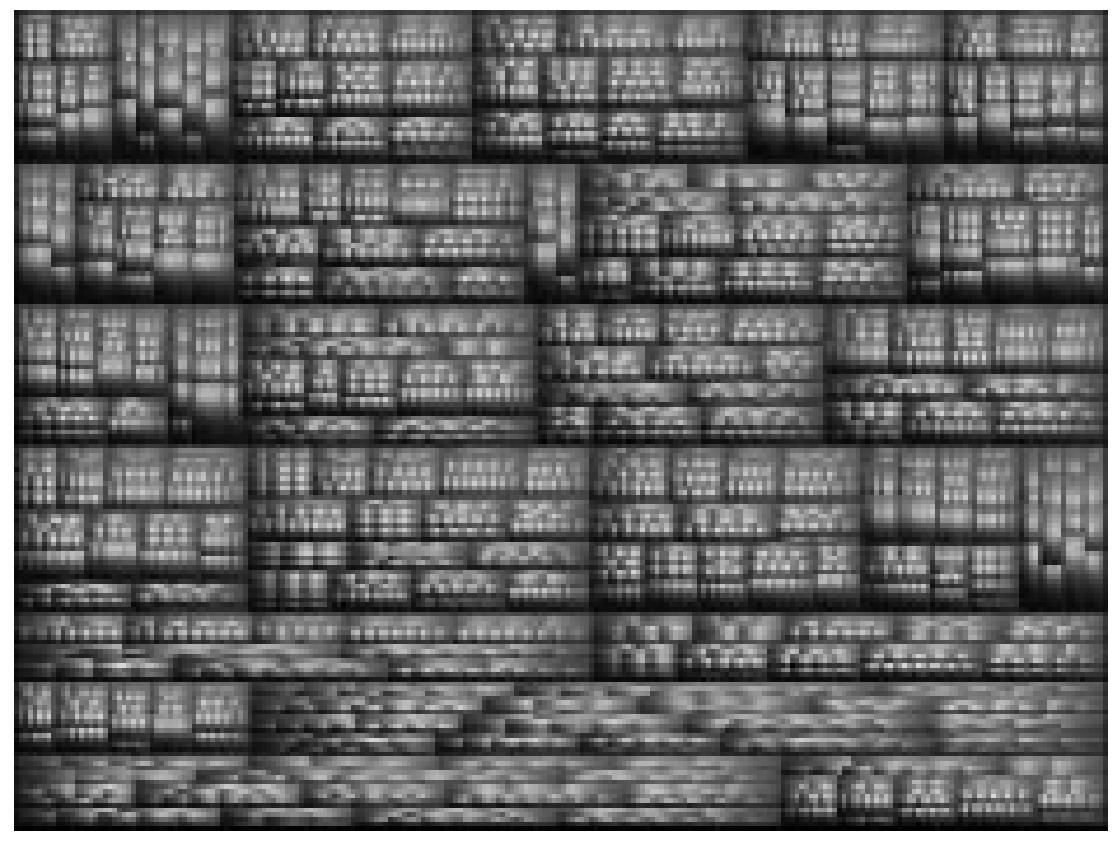
\includegraphics[width=0.8\textwidth]{images/cushionTreemap.png}
    \caption{Beispiel für eine Cushion Treemap \cite[4]{cushionTreemaps}}
    \label{fig:cushion}
\end{figure}

Peter Demian und Renate Fruchter stellen die Idee vor dass dickere outlines he höher der Knoten ist auch die Struktur verdeutlichen können. 
Nicholas Kong et al schlagen vor verschiedene Umriss dicken zu nutzen um die Struktur der Knoten darzustellen.\cite{2010-perception-treemaps} (siehe Abbildung \ref{fig:thickOutline}).
\begin{figure}
    \centering
    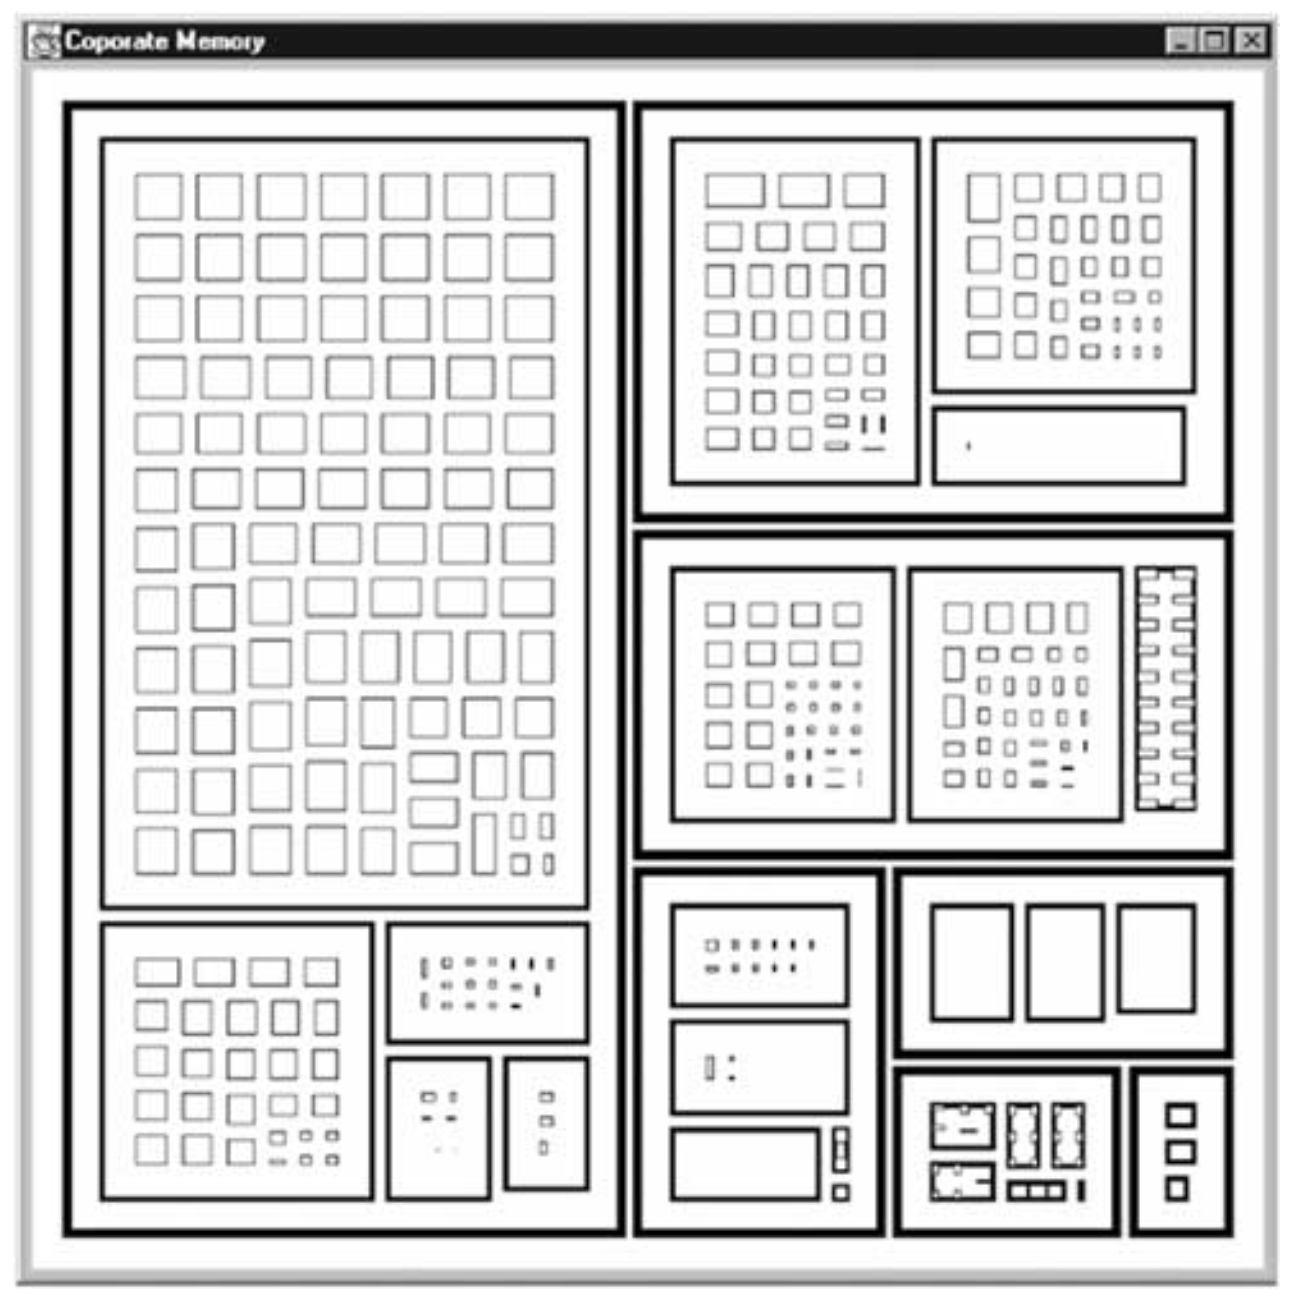
\includegraphics[width=0.8\textwidth]{images/lineThickness.png}
    \caption{Beispiel für eine Treemap mit dicken outlines, die die Struktur der Knoten verdeutlichen sollen. \cite{2010-perception-treemaps}}
    \label{fig:thickOutline}
\end{figure}

Beide Ideen sind interessant, aber für das Problem dieser Arbeit nicht relevant, da sich diese Lösungen nicht in 2.5D umsetzen lassen, da durch die Extrusion in 3D Outlines und Schatten nicht mehr Datei übergreigfend darstellt werden können.
Deshalb suchen wir hier speziell nach layouts die abstände haben. die meisten treemap layouts haben keine abstände, wodurch bei der extrusion ins drei dimensionale und ohne farbgebung die Struktur der Hierarchie nicht mehr erkennbar ist. Deswegen wird speziell nach treemap layouts gesucht, die abstände haben und die Struktur der Hierarchie darstellen.

Aktuell gibt es nur eine arbeit die dieses Problem explizit anspricht und zwar \cite{lu2008cascaded}. wir stellen diese arbeit im detail vor, da sie einige interessante Ideen hat und auch in gewisser weise einen ausgangspunkt für die in dieser Arbeit vorgestellten anpassungen an den Squarify Algorithmus darstellt.

\cite{lu2008cascaded}:
Hao Lü and James Fogarty stellten in ihrem Paper \textit{Cascaded Treemaps:
Examining the Visibility and Stability of Structure in Treemaps}\cite{lu2008cascaded} fest: \enquote{an important limitation of treemaps is
the difficulty of discerning the structure of a hierarchy}\cite[1]{lu2008cascaded} Das stellt im Grunde das Problem von Treemaps dar, welches auch algorithmisch nicht einfach gelöst werden kann (siehe Abschnitt \ref{sec:TreemapProblem}). Die Idee ist anders als bei Nested Ansätzen die Kindknoten nicht einfach in den Elternknoten zu zeichnen, sondern sie leicht versetzt \textit{über} dem Elternknoten zu zeichnen (siehe Abbildung \ref{fig:cascaded}). Dadurch soll weniger Platz verloren gehen und es entsteht ein leichter 3D-Effekt.

\begin{figure}
    \centering
    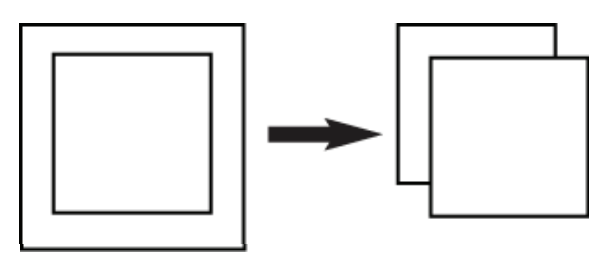
\includegraphics[width=0.8\textwidth]{images/cascaded.png}
    \caption{Links beispielhaf der Nested treemaps Ansatz, bei dem der Kindknoten einfach in dem Elternknoten gezeichnet wird. Rechts der Cascaded Treemap Ansatz, bei dem der Kindknoten als rechteck leicht versetzt nach rechts unten \textit{über} dem Elternknoten gezeichnet wird. Abbildung aus \cite[3]{lu2008cascaded}.}
    \label{fig:cascaded}
\end{figure}

Sie stellen in ihrem Paper auch fest, dass manche Knoten verschwinden können, da der Platz der für Beschriftung und abstände benötigt wird, beim Layoutschritt nicht berücksichtigt werden kann. Sie stellen einen Zwei Schrittigen ansatz vor, der im ersten schritt mit den squarify algorithmus \cite{bruls2000squarified} das layout erstellt. 
Im zweiten Schritt wird dann die Größe, aber nicht die Platzierung der Knoten angepasst. 
indem der Abstand und platz für Beschriftung berücksichtigt wird. Das Problem von verschwindenden Knoten wird dadurch nicht komplett gelöst, aber Knoten verschwinden nur noch, wenn der Platz für die Beschriftung und den Abstand größer ist als der zur Verfügung stehende Platz. Die Autoren geben leider keinen Pseudo-Code für die exakte implementierung an, weshalb es schwer ist die genaue berechnung nachzuvollziehen und Unterschiede und Vor- und Nachteile zu den Implementierungen in diser Arbeit aufzuzeigen.
Sie beschreiben ihren Schritt wie folgt: 
\begin{quote}
    The function then computes how much vertical space is needed for offsets [...]. The remaining space is for the content of the treemap, and so the layout function gives each side of the split the space computed as necessary for [...] offsets as well as a portion of the remaining content space based on the relative weights of nodes on each side of the split. The layout procedure is then ready to recurse on both sides of the split, as it knows how much space will be used by [...] offsets and has ensured that the remaining space is appropriately divided by node weight. \cite[6]{lu2008cascaded}
\end{quote} (FÜR MICH: das ist quasi simple-increase mit scaling)
Sie berechnen also die Fläche, für jeden Knoten neu. An jeder Teilungs-Kante, die kante an der ein Knoten geteilt wurde (entweder horizontal oder vertikal) - im grunde werden sich immer die reihen angeschaut. Wird dann der Platz berechnet, der für die Abstände benötigt wird. Anschließend wird der Platz für die Knoten berechnet, indem der Platz für die Abstände von der Gesamtfläche abgezogen wird. Dadurch wird sichergestellt, dass jeder Knoten genug Platz für die Abstände hat. Dennoch kann es passieren, dass Knoten verschwinden, wenn der Platz für die Abstände größer ist als der Platz, der für die Knoten zur Verfügung steht.
Obwohl der Code nicht verfügbar ist, wird doch allein bei der Beschreibung ein Nachteil deutlich: Es wird an jeder Reihen-Kante nur der Platz mit in die Berechnung einbezogen, der senkrecht zu der Kante steht. In Abbildung \ref{fig:cascadedBadExample} für deutlich, dass der Algorithmus für den Bereich über von der Kante benauso viel Platz für die Abstände berechnet, wie für den Bereicht unter der Kante, weil eben nur der Platz senkrecht zur Kante betrachtet wird. Und das obwohl offentlich die Roten Rechtecke zusammen viel Mehr platz für die Abstände benötigen würden, als das Gelbe Rechteck alleine. 
Das Grundlegende Problem, welches wir zuvor beschrieben haben (siehe Abschnitt \ref{sec:TreemapProblem}), ist also nicht gelöst. 

\begin{figure}
    \centering
    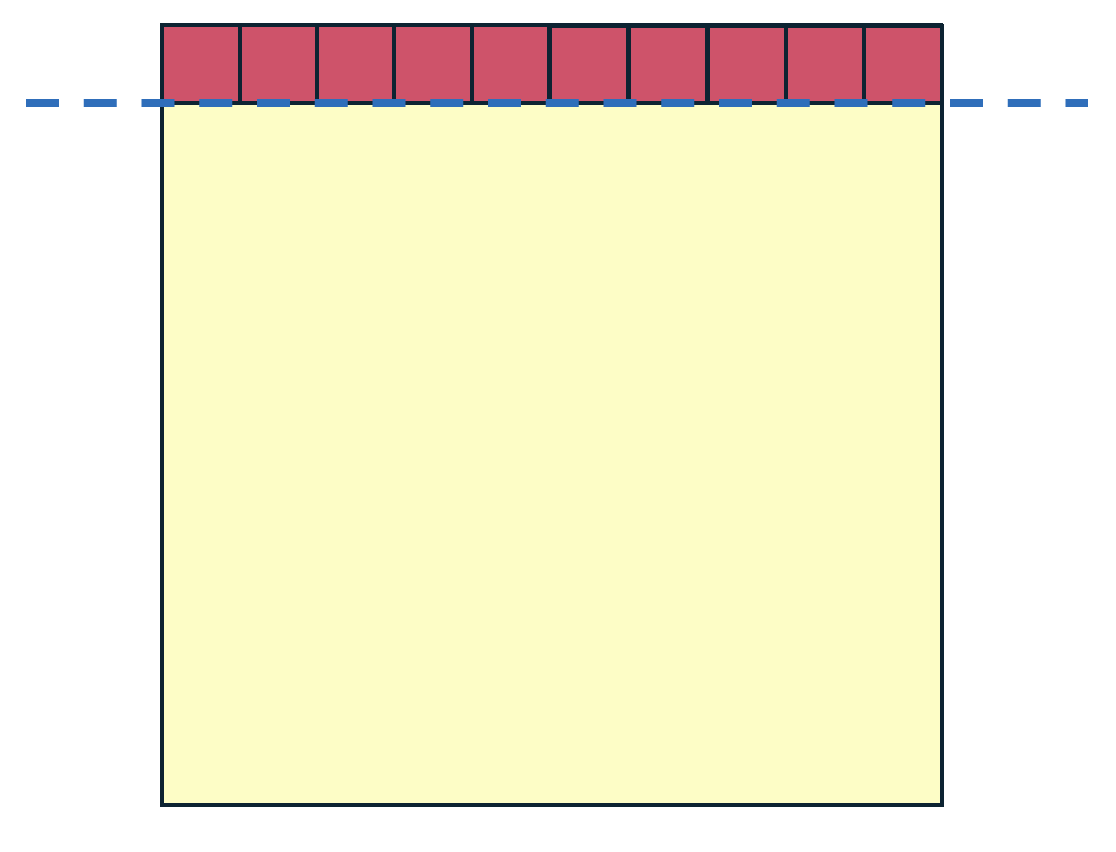
\includegraphics[width=0.8\textwidth]{images/cascadedBadExample.png}
    \caption{Beispiel für eine für den Cascaded Treemap Algorithmus schlechte Rechteck-Konstelation}
    \label{fig:cascadedBadExample}
\end{figure}

Interessant ist, dass die Autoren keine verbesserung in der Gewicht zu Größe relation feststellen konnten. (Ich vermute, dass das daran liegt, dass die Berechnung der neuen Größen für die Knoten nicht optimal ist) 
Eine verbesserung konnten sie nur bei relativ kleinen Knoten feststellen, was auch klar ist, da bei den ansätzen zuvor die Abstände (da diese ja absolut sind und bei jedem knoten gleich) die Größe von kleinen Knoten viel stärker beeinflussen, als die Größe von großen. Sie vermuten auch, dass das an Ihrem Ansatz speziell liegen könnte und fordern noch weitere research in diesem Bereich.
Sie vermuten außerdem, dass speziell bei Tiefen Hierarchien, die Abweichung von Größe zu Gewicht größer wird.  





